\usepackage{color}
\usepackage{amsmath}
\usepackage{graphicx}
%%
\title{
\jtitle{20XX年度人工知能学会全国大会・\LaTeX{}スタイルファイル}
\etitle{\LaTeX{} Style file for manuscripts of JSAI 20XX}
}
%%英文は以下を使用
%\title{Style file for manuscripts of JSAI 20XX}

\jaddress{ 相良博喜,九州大学 数理学府,福岡県福岡市西区元岡744,sagara.hiroki.043@s.kyushu-u.ac.jp }

\author{%
\jname{相良博喜\first}
\ename{Hiroki Sagara}
\and
\jname{屋藤翔麻\second}
\ename{Shoma Yato}
\and
\jname{草場壽一\third}
\ename{Shuichi Kusaba}
%\and
%Given-name Surname\third{}%%英文は左を使用
}

\affiliate{
\jname{\first{}九州大学}
\ename{Kyushu University}
\and
\jname{\second{}東京工芸大学}
\ename{Tokyo Polytechnic University}
\and
\jname{\third{}東京大学}
\ename{University of Tokyo}
}

%%
%\Vol{28}        %% <-- 28th(変更しないでください)
%\session{0A0-00}%% <-- 講演ID(必須)

\begin{abstract}
We propose a method to enhance exploration efficiency in reinforcement learning environments with sparse rewards by improving intrinsic motivation and contrastive learning. Intrinsic motivation is used to guide agents to novel states by providing internal rewards based on prediction errors. However, existing methods such as Random Network Distillation (RND) suffer from declining intrinsic rewards over time, leading to limited exploration in later stages. To address this, we introduce two modifications: (1) adjusting intrinsic rewards when episodes terminate due to agent failure, and (2) enhancing contrastive learning by treating temporally adjacent frames as positive examples. These modifications improve novelty detection and encourage consistent exploration. Experiments in sparse-reward environments such as Climber demonstrate significant improvements, with our method achieving external rewards in half the training steps compared to baseline models. Our approach maintains high intrinsic reward peaks throughout training, paving the way for more effective exploration in challenging environments.
\end{abstract}

%\setcounter{page}{1}
\def\Style{``jsaiac.sty''}
\def\BibTeX{{\rm B\kern-.05em{\sc i\kern-.025em b}\kern-.08em%
 T\kern-.1667em\lower.7ex\hbox{E}\kern-.125emX}}
\def\JBibTeX{\leavevmode\lower .6ex\hbox{J}\kern-0.15em\BibTeX}
\def\LaTeXe{\LaTeX\kern.15em2$_{\textstyle\varepsilon}$}

\begin{document}
\maketitle

\section{研究背景・目的}
強化学習(Reinforcement Learning; RL)の分野は過去10年間で目覚ましい成功を収め、多様なタスクへの対応、意思決定から複雑なゲームの習得に至るまで、その応用範囲を広げてきた。これらの進展は、計算能力の向上と機械学習手法、特にディープラーニングのブレークスルーによって推進されてきた。しかし、報酬信号が希薄な環境における効率的な探索は依然として大きな課題である。このような環境では、エージェントが複雑な状態空間を効率的にナビゲートし、限られたフィードバックから学習する能力が求められる。この問題に対する有望な解決策として、内発的動機(Intrinsic Motivation; IM)が挙げられる。IMは、新奇性や驚きなどの内部信号を活用して探索を導き、学習効率を高める。
この分野で注目すべき研究の一つが、Random Network Distillation(RND)である。RNDは、新奇性検出に基づく手法であり、固定されたランダムなターゲットネットワークと予測モデルを用いることで、エージェントに探索の指標となる内発的報酬を提供する。具体的には、予測モデルがターゲットネットワークの出力を模倣しようとする際に生じる誤差を、新奇性の指標として用いる。この手法は、報酬が希薄な環境で一定の成功を収めたが、固定されたターゲットネットワークに依存するため、内発的報酬の多様性が低く、学習が進むにつれて動機付け信号が消失するという課題がある。
こうした課題を克服するために提案されたのが、Self-supervised Network Distillation(SND)である。SNDは、ターゲットネットワークを自己教師あり学習によって動的に学習させることで、ターゲットモデルの表現を適応的に進化させ、新奇性検出の精度を向上させる。SNDは、RNDの一般化された形として位置づけられ、より高い性能と柔軟性を実現した。本研究では、このSNDフレームワークをさらに改良するために2つの取り組みを行った。
最初の取り組みは、内発的動機に基づく行動において、エピソード終了時の挙動を調整するためのηの最適化である。内発的動機に基づく行動は、新たな状態に対して無作為に取り組むため、短期間で敵と衝突するなどしてエピソードが終了してしまい、効率的な学習が妨げられる可能性がある。これに対処するため、高い内発的動機によってエピソードが終了した場合、その内発的動機に基づく報酬にマイナスの補正を加える方法を試みた。
しかし、このアプローチでは、学習に要するステップ数の短縮やパフォーマンスの顕著な向上には繋がらなかった。これにより、次の改良に焦点を移した。
2つ目の取り組みは、内発的動機の学習方法を見直すことである。特に対照学習を行う際、Noisy TV問題が発生することを考慮した。この問題は、エージェントが一時的な新奇性に過度に引き付けられ、環境の本質的な目標から注意が逸れる現象を指す。たとえば、Pitfallのようなゲームでは、NPCが点滅するブリンクやランダムな動作がエージェントの関心を不適切に引きつける可能性がある。他の環境でも、初期状態におけるランダムなキャラクターの無作為な前後移動がノイズとして作用し、エージェントの探索効率を妨げる可能性がある。
これらの問題に対処するため、対照学習を行う際に前後フレームを考慮し、連続するフレームを同一の状態として学習させる手法を導入した。この方法により、初期状態でのランダムな動作や視覚的なノイズをエージェントの興味の対象から外し、より本質的な違いに基づく状態に関心を移すことが可能となった。このアプローチにより、より短期間で報酬を得ることができ、探索効率の向上が実現した。
我々の実験では、これらの取り組みが探索効率と報酬取得の改善に寄与することを確認した。ProcGenなどの困難なゲーム環境でテストを行った結果、Noisy TV問題を効果的に緩和しベースラインモデルと比較して優れたパフォーマンスを示した。我々の手法は、特に初期状態でのランダムなノイズの影響を軽減し、エージェントが重要な状態遷移を識別し、効率的に活用する能力を向上させた。

\section{関連研究}

\section{提案手法}
\subsection{SNDの基本的な手法}
SNDは、内発的動機付けを活用し、報酬が希薄な環境における探索効率を向上させる手法である。
具体的には、強化学習における報酬に、内発的報酬\(r^{\text{intr}}\)と外的報酬\(r^{\text{ext}}\)の合成を用いて、新奇性の高い行動へエージェントを誘導する。
\[
 r_t = r^{\text{ext}}_{t} + \eta \cdot r^{\text{intr}}_{t}
\]
ここで、\(\eta\)は内発的報酬の重み付け係数である。
\begin{figure}[t]
   \centering
   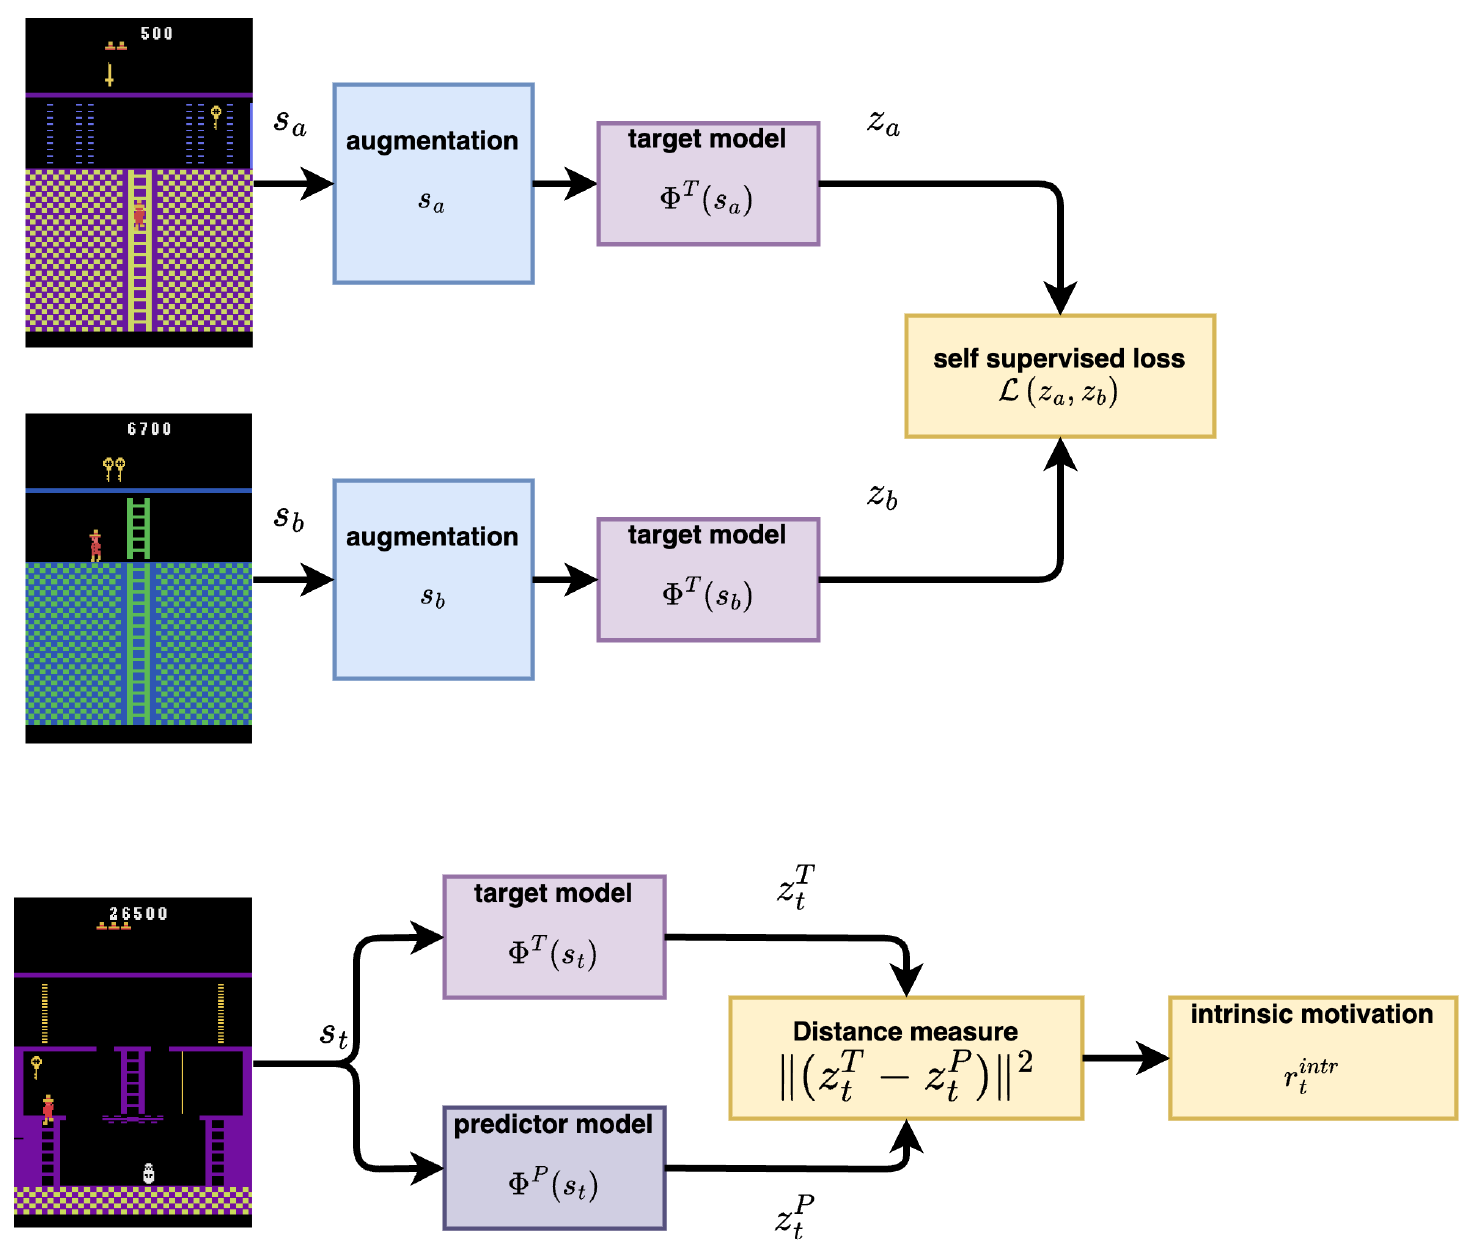
\includegraphics[width=0.5\textwidth]{figure1.eps}
   \caption{自己教師ありネットワーク蒸留(SND)の原理。提案手法は2つの主要な部分で構成されている。上部:ターゲットモデルに適した特徴の自己教師あり学習。下部:ターゲットモデルの蒸留による内的報酬の計算。本図は\cite{引用元}より転載。}\label{fig:figure1}
\end{figure}
\begin{figure}[t]
   \centering
   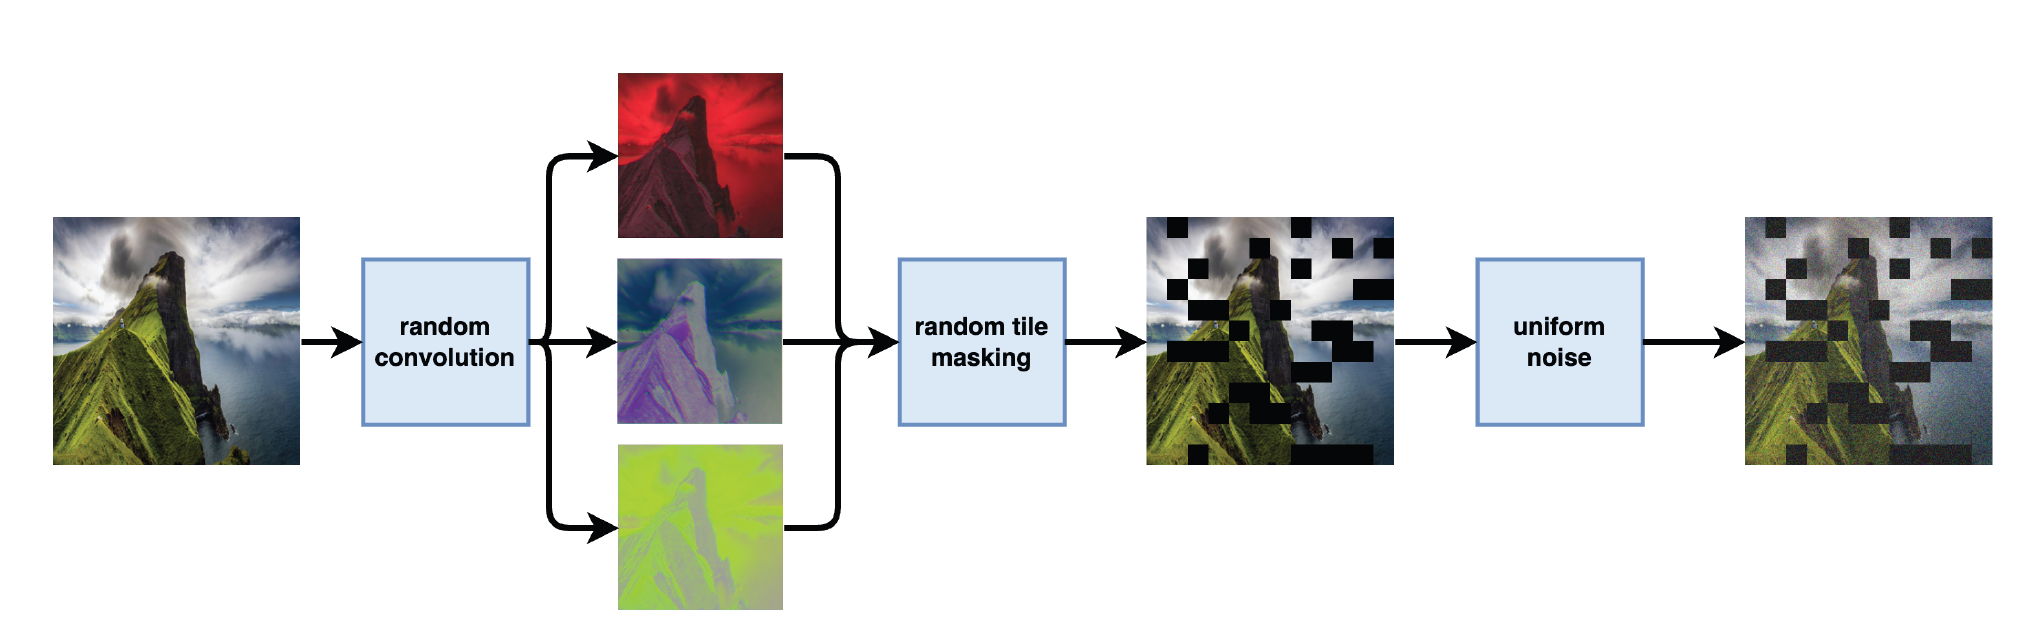
\includegraphics[width=0.5\textwidth]{figure2.eps}
   \caption{SND-Vのデータオーグメンテーション方法 本図は\cite{引用元}より転載。}\label{fig:figure2}
\end{figure}


内発的報酬は、予測モデル\(\Phi_P\)とターゲットモデル\(\Phi_T\)の間の誤差を内発的報酬として利用する。[図1]
この誤差は以下の式で定義される:
\[
 r^{\text{intr}}_{t} = \| \Phi_T(s_t) - \Phi_P(s_t) \|_2^2,
\]
ここで、\(s_t\)は現在の状態を表し、\(\|\cdot\|_2^2\)はL2ノルムの2乗を意味する。この誤差は、新奇性を評価する指標として利用され、新しい状態ほど大きな値を取る。
予測モデルは、以下の損失関数で定義される通り、ターゲットモデルの出力を模倣するよう学習が行われる。
\[
 L_P = \frac{1}{N} \sum_{s \in S} \| \Phi_T(s) - \Phi_P(s) \|_2^2,
\]
つまり、RNDのようにターゲットモデルが固定されたアルゴリズムの場合、最終的には内発的報酬が収束してしまい内発的報酬が発生しなくなる。
SNDでは、自己教師あり学習を利用してターゲットモデルを動的に更新し、状態表現の分散性を向上させる。
本研究では既往論文にて提案されているSND-Vというアルゴリズムを用いた。

\subsection{SND-V}
SND-Vは対照学習をベースとした新奇性検出手法である。
類似する状態の特徴を近づけ、異なる状態を分離する損失関数を用いることで、特徴空間を効果的に構築する。
また、状態にノイズを付与することで、ロバストな特徴表現を学習することができる。

SND-Vにおける損失関数の定義は以下の通りである:
\[
 L_T = \sum_{n} (\tau_n - \| Z_n - Z'_n \|_2^2)^2,
\]
ただし、\(\tau_n = 0\)の場合、\(Z_n\)および\(Z'_n\)は同じ状態に対してノイズを付与した状態に対する特徴ベクトルを表す。
\(\tau_n = 1\)の場合、\(Z_n\)および\(Z'_n\)は全く異なる状態、異なるエピソード、異なるステップに対してノイズを付与した状態に対する特徴ベクトルである。

ノイズの付与方法は既往研究と同様に、以下の手法を用いた。[図2]

- 一様ランダムノイズ:ピクセル値に\([-0.2, 0.2]\)の範囲でノイズを追加。
- ランダムマスキング:画像タイルをランダムにマスクする(タイルサイズは2、4、8、12、16ピクセル)。
- ランダム畳み込み:ランダムフィルターを用いた畳み込みを適用。

\subsection{提案する改良手法}
本研究では、SNDの基本的な枠組みに加え、探索効率および報酬取得の向上を目指して以下の2つの改良手法を提案する。

\subsection{改善手法1:エピソード終了時の報酬調整}

エピソード終了時における新たなルールを導入した。具体的には、エピソード終了時に\(\text{level\_complete} = \text{false}\)かつゲーム終了までのステップ数に到達していない場合、その状態を"死亡"とみなす。この場合、報酬は以下のように定義される:
\[
 r_t = \begin{cases}
 r_{\text{ext}, t} - \eta \cdot r_{\text{intr}, t}, & \text{死亡の場合},\\
 r_{\text{ext}, t} + \eta \cdot r_{\text{intr}, t}, & \text{それ以外の場合}.
\end{cases}
\]
内発的報酬が大きい状況にて死亡が発生した場合、その行動がエージェントの継続的な探索を妨げてしまっていると考えられる。このため、死亡時に内発的報酬にマイナスの補正を加えることで、エージェントがより長期的に探索を行うことができ、効率的な学習が可能となることが期待される。


\subsection{類似状態ペア選択方法の改善}
前章で述べた通り、Noisy TV問題とはエージェントが時系列的なノイズに不適切に関心を持ち、探索が非効率化する現象を指す。この問題を解決するため、SND-Vに下記の改良を加えた。

1. 同一環境およびSTEPが\(-N\)から\(+N\)ステップの範囲内にある\(2N+1\)個の状態からランダムに選択する。

2. 選択した状態にノイズを加え、類似状態ペアを構成する。

3. 非類似状態の選択は既往研究と同様にランダムに行う。

このアプローチでは、元のSND-Vが従来採用していた完全に同一の状態ペアからノイズを加える方式よりも多様な状態表現を学習できる。特に周期的に変化する状態を同一状態と捉え、無駄な内発的報酬の発生を抑えることが期待される。これにより、状態空間全体でより精度の高い新奇性検出が可能となり、エージェントが短期的なノイズではなく本質的な環境変化に基づいて行動できるようになる。

\section{実験・考察}

\subsection{実験設定}
本研究では、既往研究[x]の条件設定を引き継ぎ、提案手法の有効性を検証した。具体的には、ProcGenベンチマークのClimber環境において、提案手法を適用し、探索効率および報酬取得の改善を評価した。

\subsection{改善手法1:エピソード終了時の報酬調整}
まず、エピソード終了時の報酬調整の効果を検証した。[図3]
\begin{figure}[t]
   \centering
   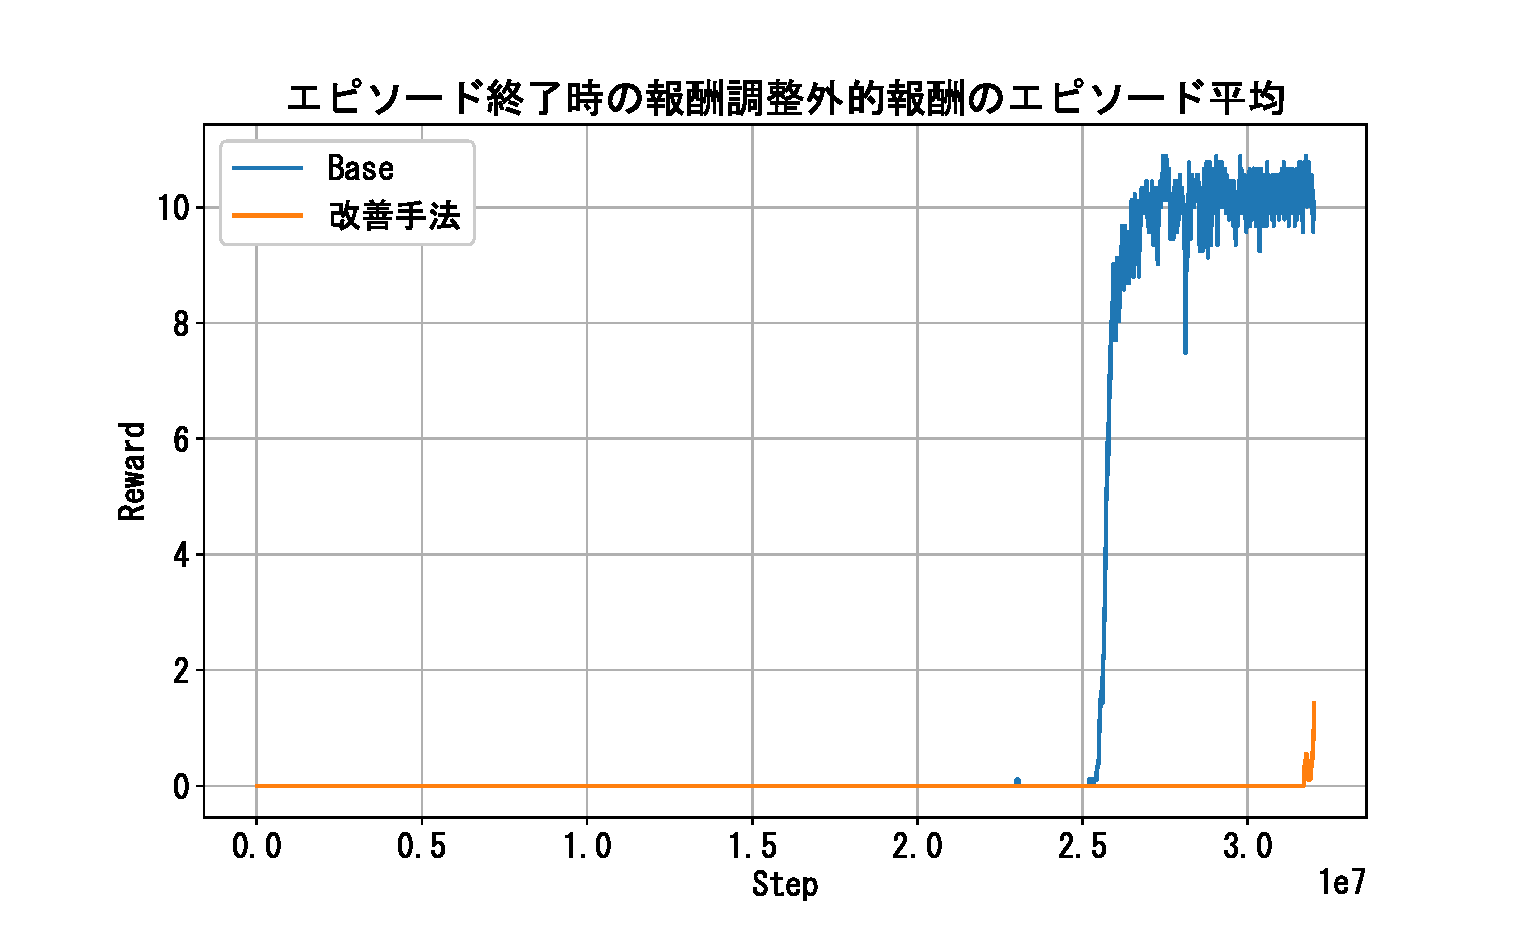
\includegraphics[width=0.5\textwidth]{Method1_Ext.eps}
   \caption{改善手法1:エピソード終了時の報酬調整 外的報酬の推移}\label{fig:figure2}
\end{figure}
\begin{figure}[t]
   \centering
   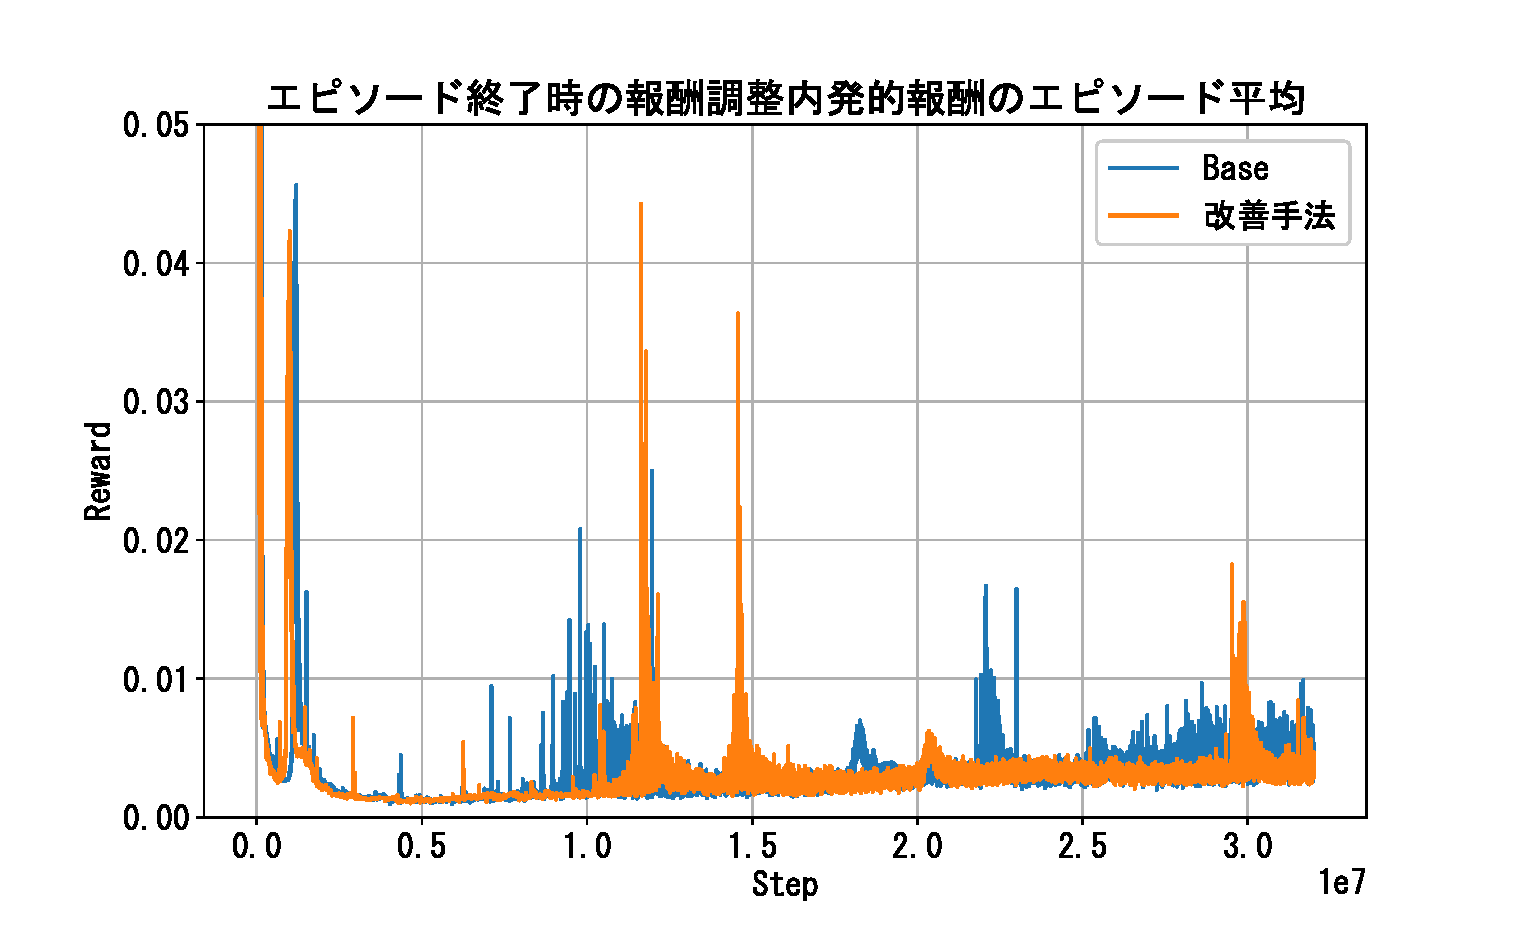
\includegraphics[width=0.5\textwidth]{Method1_Intr.eps}
   \caption{改善手法1:エピソード終了時の報酬調整 外的報酬の推移}\label{fig:figure2}
\end{figure}

結果から、提案手法が既往研究のモデルより外部報酬を得るまでの時間が長くなっていることがわかる。
また、内発的報酬に関しても、既往研究のモデルよりもピークの発生回数が少なく、内発的動機による行動が発生していないことがわかる。
このような結果となった原因を分析するため、エピソード終了時までのステップ数を生存時間解析(Kaplan-Meier法)により評価した。[図4]
\begin{figure}[t]
   \centering
   \begin{minipage}{0.23\textwidth}
       \centering
       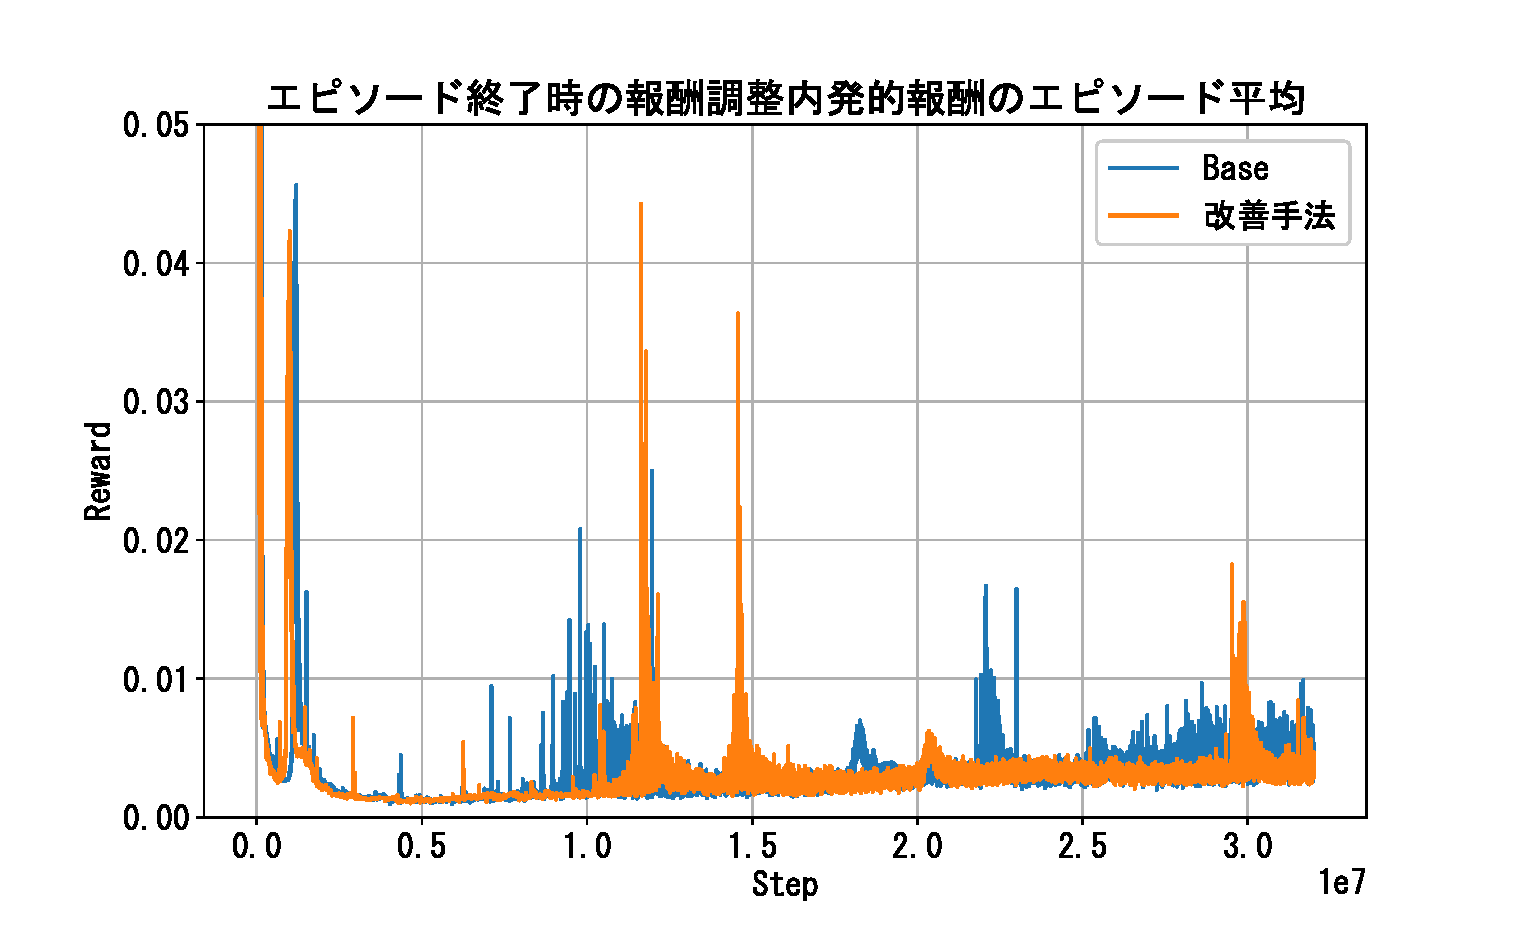
\includegraphics[width=\textwidth]{Method1_Intr.eps}
       \caption{あとで生存時間解析の図を入れる}
       \label{fig:figure1}
   \end{minipage}
   \hfill
   \begin{minipage}{0.23\textwidth}
       \centering
       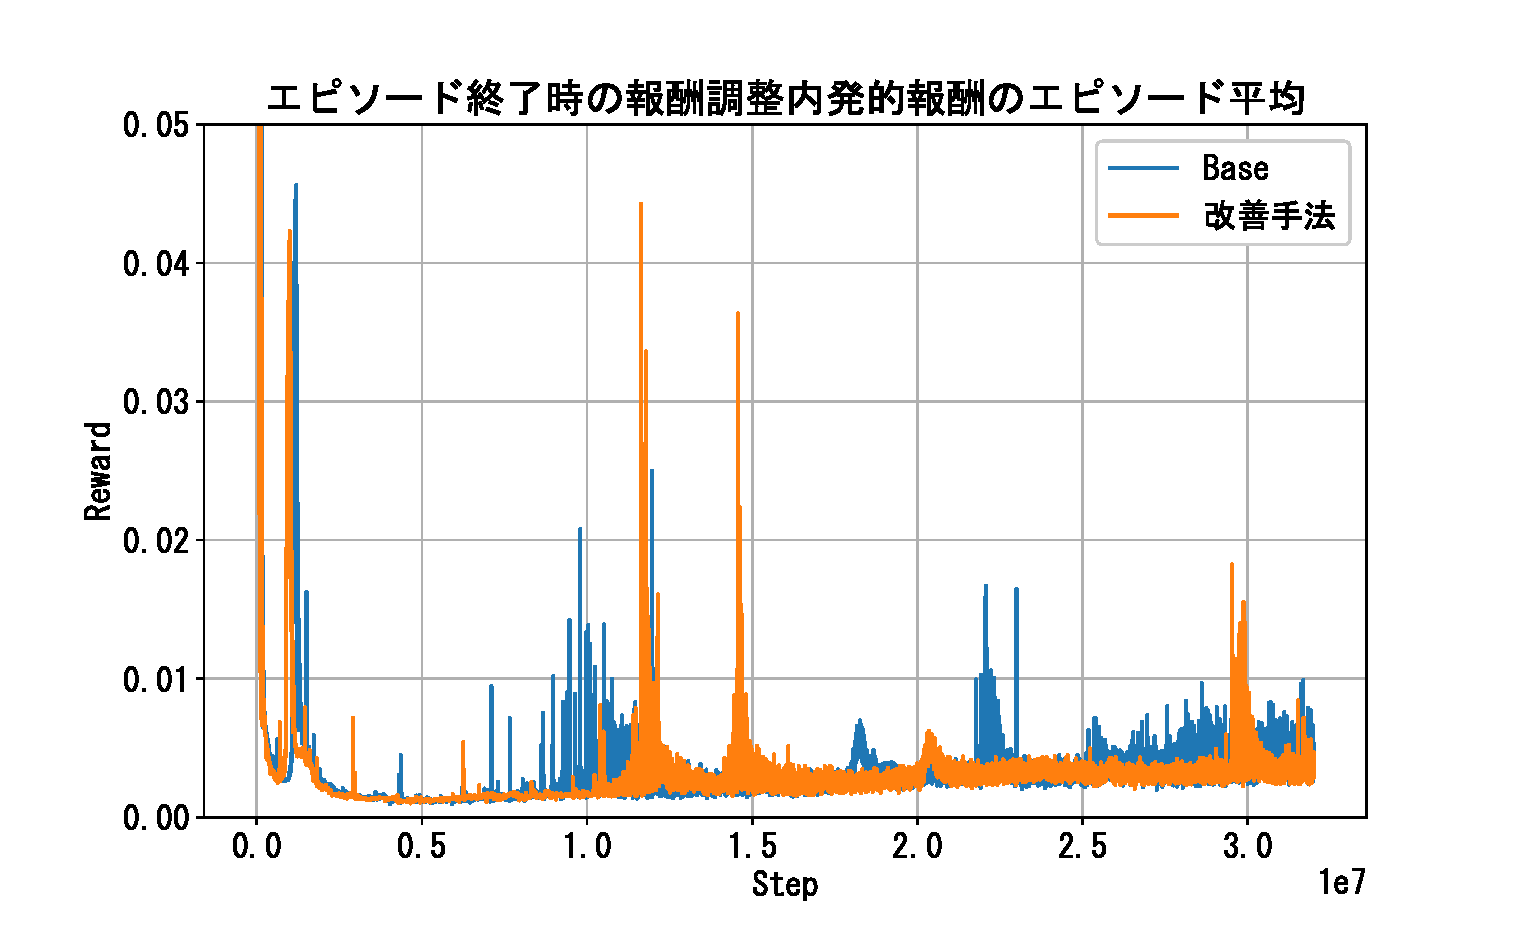
\includegraphics[width=\textwidth]{Method1_Intr.eps}
       \caption{あとで生存時間解析の図を入れる}
       \label{fig:figure2}
   \end{minipage}
\end{figure}
まだ十分に学習が進んでいない序盤に関しては、提案手法が既往研究のモデルよりも生存時間が長い。しかし、学習が進むにつれて提案手法の生存時間が短くなっていることがわかる。これは、提案手法により序盤の探索が積極的に行われず、中盤以降の学習が遅れていることを示唆していると考えられる。

\subsection{改善手法2:エピソード終了時の報酬調整}


\begin{thebibliography}{99}
\bibitem[1]{texbook}
Matej Pecháč and Michal Chovanec and Igor Farkaš, "Self-supervised network distillation: an effective approach to exploration in sparse reward environments", arXiv preprint arXiv:2106.07561, 2021
\bibitem[Lamport 86]{latexブック}
Leslie,~L: \LaTeX{}: {A} Document Preparation System (Updated for
  \LaTeX{}2$\varepsilon$), Addison-Wesley, 2nd edition (1998)
  (邦訳~: 文書処理システム \LaTeX{}2$\varepsilon$,
  阿瀬 はる美 訳, ピアソン・エデュケーション, (1999)).
\end{thebibliography}
%%
